
%% bare_jrnl.tex
%% V1.4b
%% 2015/08/26
%% by Michael Shell
%% see http://www.michaelshell.org/
%% for current contact information.
%%
%% This is a skeleton file demonstrating the use of IEEEtran.cls
%% (requires IEEEtran.cls version 1.8b or later) with an IEEE
%% journal paper.
%%
%% Support sites:
%% http://www.michaelshell.org/tex/ieeetran/
%% http://www.ctan.org/pkg/ieeetran
%% and
%% http://www.ieee.org/

%%*************************************************************************
%% Legal Notice:
%% This code is offered as-is without any warranty either expressed or
%% implied; without even the implied warranty of MERCHANTABILITY or
%% FITNESS FOR A PARTICULAR PURPOSE!
%% User assumes all risk.
%% In no event shall the IEEE or any contributor to this code be liable for
%% any damages or losses, including, but not limited to, incidental,
%% consequential, or any other damages, resulting from the use or misuse
%% of any information contained here.
%%
%% All comments are the opinions of their respective authors and are not
%% necessarily endorsed by the IEEE.
%%
%% This work is distributed under the LaTeX Project Public License (LPPL)
%% ( http://www.latex-project.org/ ) version 1.3, and may be freely used,
%% distributed and modified. A copy of the LPPL, version 1.3, is included
%% in the base LaTeX documentation of all distributions of LaTeX released
%% 2003/12/01 or later.
%% Retain all contribution notices and credits.
%% ** Modified files should be clearly indicated as such, including  **
%% ** renaming them and changing author support contact information. **
%%*************************************************************************


% *** Authors should verify (and, if needed, correct) their LaTeX system  ***
% *** with the testflow diagnostic prior to trusting their LaTeX platform ***
% *** with production work. The IEEE's font choices and paper sizes can   ***
% *** trigger bugs that do not appear when using other class files.       ***                          ***
% The testflow support page is at:
% http://www.michaelshell.org/tex/testflow/



\documentclass[journal]{IEEEtran}
%
% If IEEEtran.cls has not been installed into the LaTeX system files,
% manually specify the path to it like:
% \documentclass[journal]{../sty/IEEEtran}


\usepackage{graphicx}
\usepackage{cite}
\usepackage{color}
\def\cred{\textcolor{red}}

% Some very useful LaTeX packages include:
% (uncomment the ones you want to load)


% *** MISC UTILITY PACKAGES ***
%
%\usepackage{ifpdf}
% Heiko Oberdiek's ifpdf.sty is very useful if you need conditional
% compilation based on whether the output is pdf or dvi.
% usage:
% \ifpdf
%   % pdf code
% \else
%   % dvi code
% \fi
% The latest version of ifpdf.sty can be obtained from:
% http://www.ctan.org/pkg/ifpdf
% Also, note that IEEEtran.cls V1.7 and later provides a builtin
% \ifCLASSINFOpdf conditional that works the same way.
% When switching from latex to pdflatex and vice-versa, the compiler may
% have to be run twice to clear warning/error messages.






% *** CITATION PACKAGES ***
%
%\usepackage{cite}
% cite.sty was written by Donald Arseneau
% V1.6 and later of IEEEtran pre-defines the format of the cite.sty package
% \cite{} output to follow that of the IEEE. Loading the cite package will
% result in citation numbers being automatically sorted and properly
% "compressed/ranged". e.g., [1], [9], [2], [7], [5], [6] without using
% cite.sty will become [1], [2], [5]--[7], [9] using cite.sty. cite.sty's
% \cite will automatically add leading space, if needed. Use cite.sty's
% noadjust option (cite.sty V3.8 and later) if you want to turn this off
% such as if a citation ever needs to be enclosed in parenthesis.
% cite.sty is already installed on most LaTeX systems. Be sure and use
% version 5.0 (2009-03-20) and later if using hyperref.sty.
% The latest version can be obtained at:
% http://www.ctan.org/pkg/cite
% The documentation is contained in the cite.sty file itself.






% *** GRAPHICS RELATED PACKAGES ***
%
\ifCLASSINFOpdf
  % \usepackage[pdftex]{graphicx}
  % declare the path(s) where your graphic files are
  % \graphicspath{{../pdf/}{../jpeg/}}
  % and their extensions so you won't have to specify these with
  % every instance of \includegraphics
  % \DeclareGraphicsExtensions{.pdf,.jpeg,.png}
\else
  % or other class option (dvipsone, dvipdf, if not using dvips). graphicx
  % will default to the driver specified in the system graphics.cfg if no
  % driver is specified.
  % \usepackage[dvips]{graphicx}
  % declare the path(s) where your graphic files are
  % \graphicspath{{../eps/}}
  % and their extensions so you won't have to specify these with
  % every instance of \includegraphics
  % \DeclareGraphicsExtensions{.eps}
\fi
% graphicx was written by David Carlisle and Sebastian Rahtz. It is
% required if you want graphics, photos, etc. graphicx.sty is already
% installed on most LaTeX systems. The latest version and documentation
% can be obtained at:
% http://www.ctan.org/pkg/graphicx
% Another good source of documentation is "Using Imported Graphics in
% LaTeX2e" by Keith Reckdahl which can be found at:
% http://www.ctan.org/pkg/epslatex
%
% latex, and pdflatex in dvi mode, support graphics in encapsulated
% postscript (.eps) format. pdflatex in pdf mode supports graphics
% in .pdf, .jpeg, .png and .mps (metapost) formats. Users should ensure
% that all non-photo figures use a vector format (.eps, .pdf, .mps) and
% not a bitmapped formats (.jpeg, .png). The IEEE frowns on bitmapped formats
% which can result in "jaggedy"/blurry rendering of lines and letters as
% well as large increases in file sizes.
%
% You can find documentation about the pdfTeX application at:
% http://www.tug.org/applications/pdftex





% *** MATH PACKAGES ***
%
%\usepackage{amsmath}
% A popular package from the American Mathematical Society that provides
% many useful and powerful commands for dealing with mathematics.
%
% Note that the amsmath package sets \interdisplaylinepenalty to 10000
% thus preventing page breaks from occurring within multiline equations. Use:
%\interdisplaylinepenalty=2500
% after loading amsmath to restore such page breaks as IEEEtran.cls normally
% does. amsmath.sty is already installed on most LaTeX systems. The latest
% version and documentation can be obtained at:
% http://www.ctan.org/pkg/amsmath





% *** SPECIALIZED LIST PACKAGES ***
%
%\usepackage{algorithmic}
% algorithmic.sty was written by Peter Williams and Rogerio Brito.
% This package provides an algorithmic environment fo describing algorithms.
% You can use the algorithmic environment in-text or within a figure
% environment to provide for a floating algorithm. Do NOT use the algorithm
% floating environment provided by algorithm.sty (by the same authors) or
% algorithm2e.sty (by Christophe Fiorio) as the IEEE does not use dedicated
% algorithm float types and packages that provide these will not provide
% correct IEEE style captions. The latest version and documentation of
% algorithmic.sty can be obtained at:
% http://www.ctan.org/pkg/algorithms
% Also of interest may be the (relatively newer and more customizable)
% algorithmicx.sty package by Szasz Janos:
% http://www.ctan.org/pkg/algorithmicx




% *** ALIGNMENT PACKAGES ***
%
%\usepackage{array}
% Frank Mittelbach's and David Carlisle's array.sty patches and improves
% the standard LaTeX2e array and tabular environments to provide better
% appearance and additional user controls. As the default LaTeX2e table
% generation code is lacking to the point of almost being broken with
% respect to the quality of the end results, all users are strongly
% advised to use an enhanced (at the very least that provided by array.sty)
% set of table tools. array.sty is already installed on most systems. The
% latest version and documentation can be obtained at:
% http://www.ctan.org/pkg/array


% IEEEtran contains the IEEEeqnarray family of commands that can be used to
% generate multiline equations as well as matrices, tables, etc., of high
% quality.




% *** SUBFIGURE PACKAGES ***
%\ifCLASSOPTIONcompsoc
%  \usepackage[caption=false,font=normalsize,labelfont=sf,textfont=sf]{subfig}
%\else
%  \usepackage[caption=false,font=footnotesize]{subfig}
%\fi
% subfig.sty, written by Steven Douglas Cochran, is the modern replacement
% for subfigure.sty, the latter of which is no longer maintained and is
% incompatible with some LaTeX packages including fixltx2e. However,
% subfig.sty requires and automatically loads Axel Sommerfeldt's caption.sty
% which will override IEEEtran.cls' handling of captions and this will result
% in non-IEEE style figure/table captions. To prevent this problem, be sure
% and invoke subfig.sty's "caption=false" package option (available since
% subfig.sty version 1.3, 2005/06/28) as this is will preserve IEEEtran.cls
% handling of captions.
% Note that the Computer Society format requires a larger sans serif font
% than the serif footnote size font used in traditional IEEE formatting
% and thus the need to invoke different subfig.sty package options depending
% on whether compsoc mode has been enabled.
%
% The latest version and documentation of subfig.sty can be obtained at:
% http://www.ctan.org/pkg/subfig




% *** FLOAT PACKAGES ***
%
%\usepackage{fixltx2e}
% fixltx2e, the successor to the earlier fix2col.sty, was written by
% Frank Mittelbach and David Carlisle. This package corrects a few problems
% in the LaTeX2e kernel, the most notable of which is that in current
% LaTeX2e releases, the ordering of single and double column floats is not
% guaranteed to be preserved. Thus, an unpatched LaTeX2e can allow a
% single column figure to be placed prior to an earlier double column
% figure.
% Be aware that LaTeX2e kernels dated 2015 and later have fixltx2e.sty's
% corrections already built into the system in which case a warning will
% be issued if an attempt is made to load fixltx2e.sty as it is no longer
% needed.
% The latest version and documentation can be found at:
% http://www.ctan.org/pkg/fixltx2e


%\usepackage{stfloats}
% stfloats.sty was written by Sigitas Tolusis. This package gives LaTeX2e
% the ability to do double column floats at the bottom of the page as well
% as the top. (e.g., "\begin{figure*}[!b]" is not normally possible in
% LaTeX2e). It also provides a command:
%\fnbelowfloat
% to enable the placement of footnotes below bottom floats (the standard
% LaTeX2e kernel puts them above bottom floats). This is an invasive package
% which rewrites many portions of the LaTeX2e float routines. It may not work
% with other packages that modify the LaTeX2e float routines. The latest
% version and documentation can be obtained at:
% http://www.ctan.org/pkg/stfloats
% Do not use the stfloats baselinefloat ability as the IEEE does not allow
% \baselineskip to stretch. Authors submitting work to the IEEE should note
% that the IEEE rarely uses double column equations and that authors should try
% to avoid such use. Do not be tempted to use the cuted.sty or midfloat.sty
% packages (also by Sigitas Tolusis) as the IEEE does not format its papers in
% such ways.
% Do not attempt to use stfloats with fixltx2e as they are incompatible.
% Instead, use Morten Hogholm'a dblfloatfix which combines the features
% of both fixltx2e and stfloats:
%
% \usepackage{dblfloatfix}
% The latest version can be found at:
% http://www.ctan.org/pkg/dblfloatfix




%\ifCLASSOPTIONcaptionsoff
%  \usepackage[nomarkers]{endfloat}
% \let\MYoriglatexcaption\caption
% \renewcommand{\caption}[2][\relax]{\MYoriglatexcaption[#2]{#2}}
%\fi
% endfloat.sty was written by James Darrell McCauley, Jeff Goldberg and
% Axel Sommerfeldt. This package may be useful when used in conjunction with
% IEEEtran.cls'  captionsoff option. Some IEEE journals/societies require that
% submissions have lists of figures/tables at the end of the paper and that
% figures/tables without any captions are placed on a page by themselves at
% the end of the document. If needed, the draftcls IEEEtran class option or
% \CLASSINPUTbaselinestretch interface can be used to increase the line
% spacing as well. Be sure and use the nomarkers option of endfloat to
% prevent endfloat from "marking" where the figures would have been placed
% in the text. The two hack lines of code above are a slight modification of
% that suggested by in the endfloat docs (section 8.4.1) to ensure that
% the full captions always appear in the list of figures/tables - even if
% the user used the short optional argument of \caption[]{}.
% IEEE papers do not typically make use of \caption[]'s optional argument,
% so this should not be an issue. A similar trick can be used to disable
% captions of packages such as subfig.sty that lack options to turn off
% the subcaptions:
% For subfig.sty:
% \let\MYorigsubfloat\subfloat
% \renewcommand{\subfloat}[2][\relax]{\MYorigsubfloat[]{#2}}
% However, the above trick will not work if both optional arguments of
% the \subfloat command are used. Furthermore, there needs to be a
% description of each subfigure *somewhere* and endfloat does not add
% subfigure captions to its list of figures. Thus, the best approach is to
% avoid the use of subfigure captions (many IEEE journals avoid them anyway)
% and instead reference/explain all the subfigures within the main caption.
% The latest version of endfloat.sty and its documentation can obtained at:
% http://www.ctan.org/pkg/endfloat
%
% The IEEEtran \ifCLASSOPTIONcaptionsoff conditional can also be used
% later in the document, say, to conditionally put the References on a
% page by themselves.




% *** PDF, URL AND HYPERLINK PACKAGES ***
%
%\usepackage{url}
% url.sty was written by Donald Arseneau. It provides better support for
% handling and breaking URLs. url.sty is already installed on most LaTeX
% systems. The latest version and documentation can be obtained at:
% http://www.ctan.org/pkg/url
% Basically, \url{my_url_here}.




% *** Do not adjust lengths that control margins, column widths, etc. ***
% *** Do not use packages that alter fonts (such as pslatex).         ***
% There should be no need to do such things with IEEEtran.cls V1.6 and later.
% (Unless specifically asked to do so by the journal or conference you plan
% to submit to, of course. )


% correct bad hyphenation here
\hyphenation{op-tical net-works semi-conduc-tor}


\begin{document}
%
% paper title
% Titles are generally capitalized except for words such as a, an, and, as,
% at, but, by, for, in, nor, of, on, or, the, to and up, which are usually
% not capitalized unless they are the first or last word of the title.
% Linebreaks \\ can be used within to get better formatting as desired.
% Do not put math or special symbols in the title.
%\title{Thermal performance of a prototype polarization modulator using a superconducting magnetic bearing operating below 10 K}
\title{Estimation of the heat dissipation and the rotor temperature of superconducting magnetic bearing below 10 K}
%
%
% author names and IEEE memberships
% note positions of commas and nonbreaking spaces ( ~ ) LaTeX will not break
% a structure at a ~ so this keeps an author's name from being broken across
% two lines.
% use \thanks{} to gain access to the first footnote area
% a separate \thanks must be used for each paragraph as LaTeX2e's \thanks
% was not built to handle multiple paragraphs
%

\author{Yuki Sakurai, Tomotake Matsumura, Hirokazu Kataza, Shin Utsunomiya, Ryo Yamamoto
\thanks{Y. Sakurai and S. Utsunomiya are with University of Tokyo, Kavli-Institute of Physics, Mathematics and Universe (Kavli-IPMU), Kashiwa, Chiba, Japan, e-mail: yuki.sakurai@ipmu.jp}
\thanks{T. Matsumura, H. Kataza, R. Yamamoto are with Institute of Space and Astronautical Science (ISAS), Japan Aerospace Exploration Agency (JAXA), Sagamihara, Kanagawa 252-5210, JAPAN}
\thanks{H. Kataza is with University of Tokyo, Department of Astronomy.}
\thanks{R. Yamamoto is with University of Tokyo, Department of Physics.}
\thanks{Manuscript received September 10, 2016; revised September **, 2016.}}

% note the % following the last \IEEEmembership and also \thanks -
% these prevent an unwanted space from occurring between the last author name
% and the end of the author line. i.e., if you had this:
%
% \author{....lastname \thanks{...} \thanks{...} }
%                     ^------------^------------^----Do not want these spaces!
%
% a space would be appended to the last name and could cause every name on that
% line to be shifted left slightly. This is one of those "LaTeX things". For
% instance, "\textbf{A} \textbf{B}" will typeset as "A B" not "AB". To get
% "AB" then you have to do: "\textbf{A}\textbf{B}"
% \thanks is no different in this regard, so shield the last } of each \thanks
% that ends a line with a % and do not let a space in before the next \thanks.
% Spaces after \IEEEmembership other than the last one are OK (and needed) as
% you are supposed to have spaces between the names. For what it is worth,
% this is a minor point as most people would not even notice if the said evil
% space somehow managed to creep in.



% The paper headers
\markboth{Journal of \LaTeX\ Class Files,~Vol.~14, No.~8, August~2015}%
{Shell \MakeLowercase{\textit{et al.}}: Bare Demo of IEEEtran.cls for IEEE Journals}
% The only time the second header will appear is for the odd numbered pages
% after the title page when using the twoside option.
%
% *** Note that you probably will NOT want to include the author's ***
% *** name in the headers of peer review papers.                   ***
% You can use \ifCLASSOPTIONpeerreview for conditional compilation here if
% you desire.




% If you want to put a publisher's ID mark on the page you can do it like
% this:
%\IEEEpubid{0000--0000/00\$00.00~\copyright~2015 IEEE}
% Remember, if you use this you must call \IEEEpubidadjcol in the second
% column for its text to clear the IEEEpubid mark.



% use for special paper notices
%\IEEEspecialpapernotice{(Invited Paper)}




% make the title area
\maketitle

% As a general rule, do not put math, special symbols or citations
% in the abstract or keywords.
\begin{abstract}
We present the thermal characteristics of a superconducting magnetic bearing (SMB) system that is designed for a polarization modulator of a cosmic microwave background (CMB) polarization experiment. We have focused on two types of measurements. One is to estimate the heat dissipation from friction of the SMB. We have conducted the spin down measurements and we projected the heat dissipation of 3~mW from the hysteresis contribution. We discuss the consistency to the Bean's model between the magnetic field inhomogeneity and the hysteresis loss. We also characterize the thermal characteristics of the holder mechanism for the SMB system at below 10~K. We measure the thermal conductance of a grip holder, which is the thermal path when the rotor is held in place at the time of field cooling. The effective thermal conductance is 1~mW/K without any extra-effort to polish nor gold plate the contact surface. We also implement a technique to estimate a levitating rotor temperature by using a thermal conductance of a gripper contact. The gripper thermometer follows a temperature of the rotor. The extrapolated temperature recovers the rotor temperature with the difference of less than 2~K without any correction.
\end{abstract}

% Note that keywords are not normally used for peerreview papers.
\begin{IEEEkeywords}
Superconducting magnetic bearing
\end{IEEEkeywords}

% For peer review papers, you can put extra information on the cover
% page as needed:
% \ifCLASSOPTIONpeerreview
% \begin{center} \bfseries EDICS Category: 3-BBND \end{center}
% \fi
%
% For peerreview papers, this IEEEtran command inserts a page break and
% creates the second title. It will be ignored for other modes.
\IEEEpeerreviewmaketitle


\section{Introduction}
\IEEEPARstart{A}{} cosmic microwave background (CMB) radiation is a relic radiation from the big bang.
We can measure this radiation today as an oldest light from the universe.
One of the fundamental questions in cosmology is to probe the presence of cosmic inflation just after the beginning of the universe.
Although such this event may be happening as early as $\sim10^{-38}$ seconds after the beginning of the universe, the theory of inflation predicts the existence of the divergence free pattern in the CMB polarization, called B-mode, with the presence of inflation.
The world-wide effort to hunt this signal is in progress from ground, balloon, and space-borne telescopes, and the corresponding instrumental development is ongoing.
One of the key instruments for this type of measurements is called a polarization modulator, which consists of an optical element, a half-wave plate (HWP), that rotates at a few Hz at the cryogenic temperature.
Due to the faint signal, the HWP has to be maintained below about 10~K in order to minimize its own thermal emission.
As a result, this system requires to achieve the continuous rotation at about 10~K or below.
The standard mechanical bearing dissipates too much heat, and thus it is important to employ the rotational mechanism that allows to rotate with minimal heat dissipation at the cryogenic temperature.
A superconducting magnetic bearing (SMB) is a contactless bearing, and thus it achieves a continuous rotation at cryogenic temperature environment with minimal energy loss from friction.
This technology is particularly attractive for various applications, including flywheel energy storage and high efficiency motor bearings.
A polarization modulator for a CMB polarization experiment is one of the applications which an SMB can play a key role to enable the continuous rotation at below 10~K environment.
In the past, EBEX is a balloon-borne CMB experiment that employs an SMB system for the polarization modulator, and there is an increasing interest to apply this technology to a ground telescope and even to a satellite mission\cite{jklein}.

While the contactless bearing, like SMB, can achieve very low deceleration but not zero.
This is due to the magnetic interaction between a rotor and a stator.
Previously we have conducted an experiment to estimate the energy loss using a scaled prototype SMB model (diameter of 65~mm), and estimated the energy loss corresponds to the power dissipation of $19~\mu$W at 1~Hz under the vacuum environment below 10~K \cite{matsumura_eucas2015}.

In this paper we address the two key questions about non-zero friction of the SMB.
One is to estimate the heat dissipation due the friction from a bearing, which has an opening diameter of about 400~mm, a typical size for a CMB polarization experiment.
We have conducted a spin down measurement at room pressure using liquid nitrogen to estimate the heat dissipation.

Secondly, the energy loss from the non-zero friction will eventually become heat.
A part of the heat goes to the stator and the rest goes to the rotor.
Since the rotor of SMB does not have any physical contact once levitates, there is no direct access to measure the rotor temperature.
We implement the technique that is introduced by Klein et al. to estimate the rotor temperature and we demonstrate its functionality \cite{jklein}.

%In this paper, we address the heat dissipation and the temperature estimation of the rotor magnet experimentally using the two experimental configurations.
%First we describe the spin down measurements that is conducted at the room pressure using the liquid nitrogen.
%Second we describe the demonstration of the technique to estimate to the rotor temperature.
Finally we discuss our results and further challenges to be addressed.

\section{Heat dissipation from friction}
We prepare an SMB system that has an opening diameter of 394~mm.
The ring magnet consists of 16 segmented NdFeB magnets that is magnetized axially with the magnetic remnance of 1.24~T.
The ring shaped HTS array is formed in a ring shape using three-seeded YBCO tiles.
Both the ring magnet and the HTS tiles are fabricated by ATZ~\cite{atz}.

Because we are in preparation of a large cryostat to encase the entire system, we conducted the spin down measurements using a Styrofoam bucket with liquid nitrogen (top panel of Figure~\ref{fig:spindown}).
We measured the spin down with the two different levitation height, the gap between the bottom of the rotor and the top of the HTS, as 3~mm and 6~mm.
The rotational frequency is monitored by using an optical chopper directly mounted on the rotor and an optical encoder, LED and Silicon photo-diode.
We also mount a Hall sensor at the gap between the rotor magnet and the HTS tiles.
Thus, we monitor the magnetic field as the rotor magnet rotates during the spin down.

The bottom panel of Figure~\ref{fig:spindown} shows the rotational frequency as a function of time.
The rotor is freely spinning down at the levitation height of 6~mm.
The left panel of Figure~\ref{fig:Bval} shows the magnetic field variation as a function of the time from the same spin down measurement.
The magnetic field inhomogeneity is originated due to the two reasons: the gap between the segments and the inhomogeneity of each segment magnet itself.

We model this spin down profile as the following deceleration, $\alpha$,
\begin{eqnarray}
\alpha = 2\pi \frac{df}{dt} = a_0 + 2\pi a_1 f,
\label{eq:spindown}
\end{eqnarray}
where $f$ is the rotational frequency\cite{hull_review}.
The first term, $a_0$, represents the hysteresis loss, and the second term, $a_1$, represents the eddy current loss as well as air friction.
We believe that the fitted $a_1$ is dominated by the air friction due to the test condition.
We fit the data with Eq.~\ref{eq:spindown} and the fitted parameters are summarized in Tab.~\ref{tab:fitpar}.

We also parameterized the magnetic field inhomogeneity in two ways.
One is to compute the histogram of the magnetic field variation, fit with the Gaussian form, e$^{-(B-\bar{B})^2/2\sigma_B}$ and extract $\sigma_B^2$ as a measure of the inhomogeneity.
The other is to employ the difference between the maximum and the minimum within one period of revolution.

According to the Bean's model \cite{beans_model_1,beans_model_2}, the energy loss, $\Delta E$, due to the hysteresis is modelled as
\begin{eqnarray}
\Delta E \propto \frac{(\Delta B)^3}{J_c}
\label{eq:bean}
\end{eqnarray}
where $\Delta B$ is the magnetic field inhomogeneity and $J_c$ is the YBCO critical current.

%We compare the fitted $a_0$ and $\sigma_B$.
%We form the ratio as
The fitted $a_0$ and $\sigma_B$ are compared by taking the ratio as
\begin{eqnarray}
\frac{a_0(h=6\mbox{mm})}{a_0(h=3\mbox{mm})} / \frac{\sigma^3_B(h=6\mbox{mm})}{\sigma^3_B(h=3\mbox{mm})} = 1.3,
\label{eq:beanmodelcheck}
\end{eqnarray}
where $h$ is the levitation height.
In this comparison, we assume the $J_c$ is a constant value regardless of the levitation height.
Without any correction, the relationship between $a_0$ and $\sigma_B$ scales similar to the Bean's model.
When the magnetic field variation is quantified as
\begin{eqnarray}
\Delta B = B_{max} - B_{min},
\label{eq:bmax-bmin}
\end{eqnarray}
this definition captures the spiky features in the magnetic field.
In this case, the previously defined ratio in Eq~\ref{eq:beanmodelcheck} changes to 5.1 from 1.3.
%% appear as 5.1.
%We use the magnetic field that is measured at the fixed radial position and this radial position corresponds to the rotor magnetic field close to be maximum after the field cooled.

Our results match to the $\Delta B^3$ scaling using $\sigma_B$ instead of the difference of the magnetic field between the maximum and the minimum.
The difference of the two conventions is essentially to either include or exclude the spiky features in the magnetic field inhomogeneity.
Although this is beyond the scope of the paper, it is interesting to pursue the numerical simulation and study the hysteresis loss with the actual measured magnetic field.
The current measured magnetic field is only conducted at the single radial position.
It is more informative to measure the three dimensional magnetic field structure and provide them as an simulation input.
%The fact that the measure of the magnetic field inhomogeneity matches to the $\Delta B^3$ scaling with $\sigma_B$ as compared to the maximum minus minimum the following question.
%We identify the interesting question about what is the proper figure-of-merit to define the magnetic field variation when the rotor magnet consists of a segmented magnet and thus the gap produces a spiky magnetic field inhomogeneity.
%Also the measurement of the magnetic field relies on one radiation position and the magnetic field is not fully mapped in three dimension.
%Although it is beyond the scope of this paper, the further modelling the rotor magnetic field can provide more detailed characterizations of the magnetic field dependence to the hysteresis loss.

Given the fitted parameters, we project the heat dissipation, $P_{h}$, given the energy loss.
We only accounted $a_0$ from this measurements.
\begin{eqnarray}
P_{h} = \tau_{drag} \omega = I \alpha(a_1=0) \omega,
\label{eq:energyloss}
\end{eqnarray}
where $\omega$ is the angular speed.
The expected power dissipation due to the friction is 3~mW at the levitation height of 6~mm.
This can be realized by designing the SMB system that is run in vacuum with use of non-metallic material or slotted metal in surrounding structures to minimize the eddy current loss.
The further suppression of this power dissipation can be expected by minimizing the magnetic field inhomogeneity of the rotor magnet.
We are currently addressing this design optimization and will report in the future paper.

\begin{figure}[htb]
   \centering
   \includegraphics[width=70mm]{D400mm.eps} \\
   \vspace{3mm}
   \includegraphics[width=75mm]{spindown.eps}
   \caption{Top: The experimental setup for the spin down measurements for $D=395$~mm. Bottom: The rotational frequency as a function of time at the levitation height of 6~mm.}
   \label{fig:spindown}
\end{figure}

\begin{figure}[htb]
   \centering
   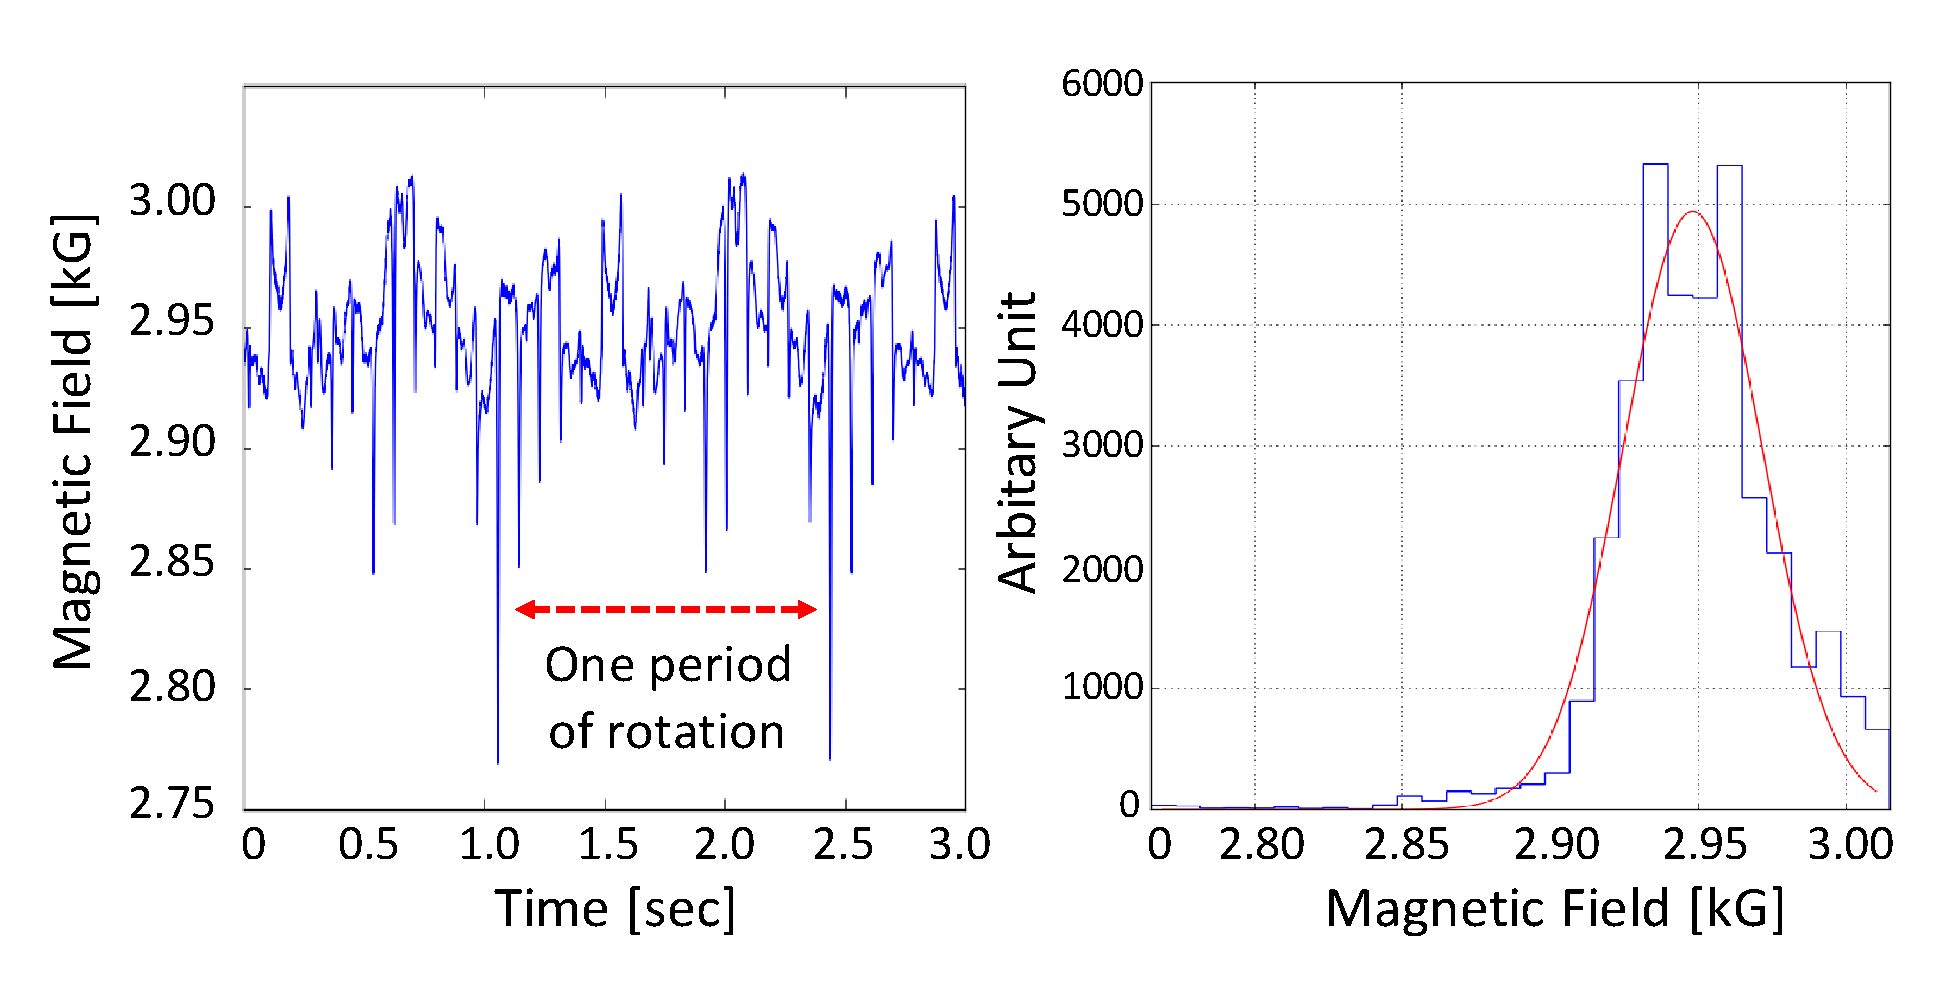
\includegraphics[width=85mm]{magneticfieldvariation_rev.eps} % requires the graphicx package
   \caption{Left: The magnetic field inhomogeneity as a function of time for $D=395$~mm SMB system at the levitation height of 6~mm. Right: The histogram of the magnetic field at the levitation height of 6~mm. The red line is the results of the Gaussian fit. }
   \label{fig:Bval}
\end{figure}


% Requires the booktabs if the memoir class is not being used
\begin{table*}[t]
   \centering
   %\topcaption{Table captions are better up top} % requires the topcapt package
   \begin{tabular}{c|c|c|c|c|c|c} % Column formatting, @{} suppresses leading/trailing space
	    $D$ & $h$& $P_p$ & $\sigma_B$ &$a_0$ & $a_1$  & $P_h$\\
	     $[\mbox{mm}]$ & $[\mbox{mm}]$ & $[\mbox{atm}]$ & $[\mbox{kG}]$ & $[\mbox{s}^{-2}]$  & $[\mbox{s}^{-2}]$  & $[\mbox{W}]$ \\ \hline
        394 & 3  & 1  & $5.7\times10^{-2}$ & $5.7\times10^{-3}$  & $1.2\times10^{-3}$ & $3.6\times10^{-2}$\\
	394 & 6  &  1 & $2.3\times10^{-2}$ & $5.1\times10^{-4}$ & $7.6\times10^{-4}$ & $3.2\times10^{-3}$\\
	65 & 6   &  $<10^{-8}$ & $2\times10^{-2}$ & $1.3\times10^{-3}$ & $2.2\times10^{-4}$ & $1.9\times10^{-5}$
   \end{tabular}
   \caption{The summary of the fit parameters from the spin down measurements and the extrapolation to the heat dissipation.
     $D$ is the inner diameter of the rotor magnet.
     $h$ is the levitation height.
     $P_p$ is the pressure at the time of the spin down measurements.
     $P_h$ is the projected heat dissipation from the $a_0$ term.}
%is the gap between the rotor magnet surface and the HTS surface.

   \label{tab:fitpar}
\end{table*}

\section{Thermal characterization of the rotor temperature}
A scaled prototype SMB system is constructed.
The detailed description of this prototype system is in Matsumura et al.~\cite{matsumura_eucas2015}.
This system is a scaled model of the SMB system that is described in the previous section, and the opening diameter of the rotor is 65~mm.
The entire system is enclosed in a GM cryostat and is cooled down to the lowest temperature of about 6~K.

The cooling sequence is following.
The rotor magnet is held by the three grippers when the SMB is cooled from the room temperature to about 6~K.
The YBCO array is field-cooled by the magnetic field of the rotor.
Once the rotor is thermalized by conduction through the three gripper arms, the rotor is released and it levitates.

\subsection{Thermal conductivity of the holder mechanism}
The thermal conductance between the stator and the rotor during the cool down process is purely limited by the physical contact of the holder mechanism.
The three grippers are placed in 120 degrees apart as shown in Figure~\ref{fig:figureA}.
Each gripper has a wedge shape that moves radially and mate with the rotor that also has an identical but negative wedge shape.
The gripper is actuated by a cryogenic stepping motor.
We mounted a temperature sensor on the gripper arm.
We also placed three heaters, thin-film resistors, on the rotor.
The thermal conductance via wires for the thermometers and heaters are estimated as less than 6~$\mu$W.
We measure the temperature difference between the rotor and the gripper arm.
Figure~\ref{fig:thermalcond} shows the linear relationship between the applied electrical heat and the temperature difference between the rotor and the gripper arm.
We derive the effective thermal resistance between the two temperature sensors, including two metal surfaces, from the slope.
The thermal resistance is $10^{3}$~K/W, and the corresponding effective thermal conductance is $1$~mW/K.
The gripper arm and the rotor holder is made of aluminum.
The surfaces of the gripper and the rotor are not polished nor gold plated, and thus there is a room for improvement.
While we can increase the pressure between the two surfaces by applying more torque to the gripper against to the rotor we did not pursue this in order to mitigate the actuator to be stacked by applying too much torque.

%The three thin-film resistors (heater) and the three temperature sensor (Cernox) are mounted on the rotor. The resistive power is applied when the rotor magnet is held by the three grippers and we estimate the thermal conductance through the physical contact of the holder mechanism.
%Once the rotor is levitating, the rotor temperature is difficult to estimate. We develop the calibration scheme to estimate the rotor temperature by using a thermometer mounted at the gripper arm.

\begin{figure}[htb]
   \centering
   \includegraphics[width=90mm]{figureA_rev.eps} % requires the graphicx package
   \caption{Top: a cross-sectional view of the gripper and the rotor. Bottom right: The top view of the rotor and the three grippers. Bottom left: The gripper.}
   \label{fig:figureA}
\end{figure}

\begin{figure}[htb]
   \centering
   \includegraphics[width=80mm]{thermalcond.eps} % requires the graphicx package
   \caption{The relationship between the applied power and the temperature difference between the rotor and the gripper arm. }
   \label{fig:thermalcond}
\end{figure}

\begin{figure}[htb]
   \centering
   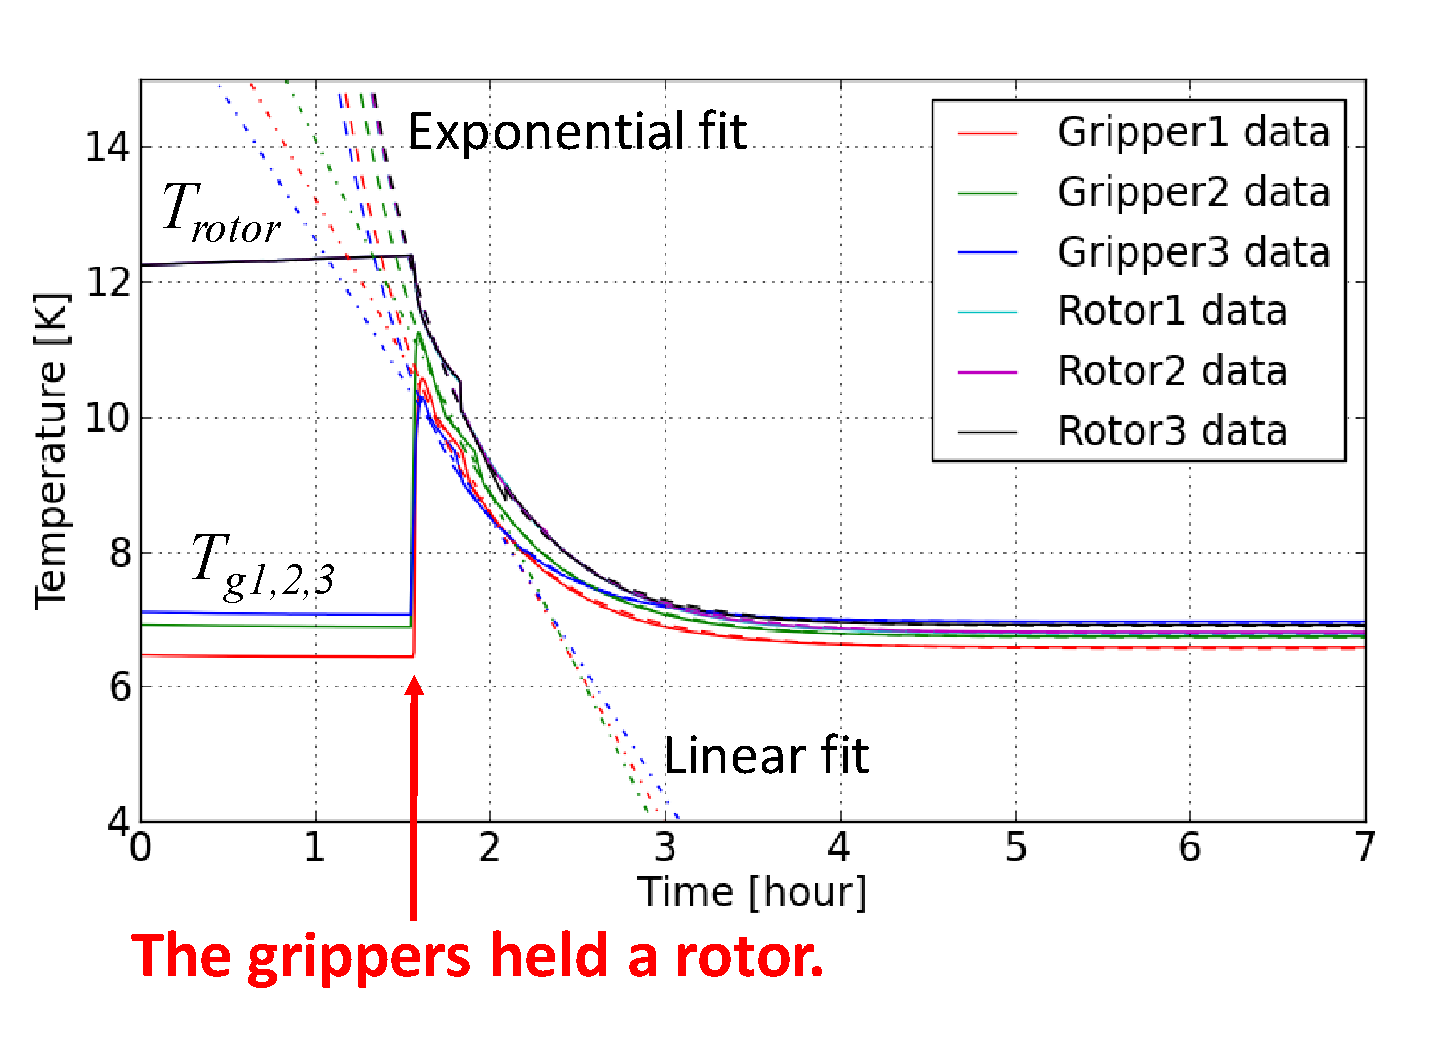
\includegraphics[width=80mm]{TemperatureEstimate_rev.eps} % requires the graphicx package
   \caption{The temperature profile of the grippers and the rotor as a function of time. }
   \label{fig:TemperatureEstimate}
\end{figure}

\subsection{Estimation of the rotor temperature}
When a rotor is levitating, it is difficult to estimate its temperature remotely.
We conduct an experiment to estimate the rotor temperature by monitoring the temperature on the gripper arm at the moment of grabbing the rotor.
The sequence of the experiment is following.
The three grippers hold the rotor until the rotor is thermalized.
%Once the rotor is thermalized,
Then, the rotor is released from the three grippers and thus the rotor levitates.
We apply the electrical power to the rotor heater.
The rotor temperature increases due to no thermal pass except the radiation and resistive wires.
Once the temperature of the rotor increases to about 10~K, the rotor is grabbed using the grippers.
%we grip the rotor using the three grippers.
We monitor the temperature rise of the three temperature sensors mounted on each gripper arm.

Figure~\ref{fig:TemperatureEstimate} shows the temperature profile as a function of time.
The gripper temperature spikes up when the gripper makes a contact to the rotor.
The rotor temperature starts decreasing together with the gripper temperature once the gripper temperature reaches to maximum.
We fit the gripper temperature data with two functional forms, linear and exponential.
When the temperature difference between the stator and the levitating rotor is small, the exponential form fits well.
On the other hand, the temperature difference is large, the linear function fits better.
For the linear fit, we select the gripper temperature data between $T_g^{max}$ and$(T_g^{max}+T_g^{min})/2$,
where $T_g^{max}$ and $T_g^{min}$ are the maximum and the minimum temperature of the gripper in this profile.

The reason why we choose the two functional forms are followings.
If the specific heat and the thermal conductivity of the gripper and the rotor are constant with a temperature, the temperature profile in Figure~\ref{fig:TemperatureEstimate} is expected to be an exponential functional form.
As the temperature change is significant enough to take into account the temperature dependence of the thermal conductivity and the specific heat, the temperature profile is expected to be linear.
%The temperature decreasing is expected to depend on the specific heat and the thermal conductivity of the gripper arm and the rotor holder.
%The specific heat and the thermal conductivity are possible to vary with temperature and the pressure between two surfaces of the gripper and the rotor holder.

The extrapolated temperature from the fit at the time of the gripping shows the lower temperature than the actual rotor temperature by less than 2~K, even if we use either of the fit functions.

\section{Conclusion}
We have conducted two experiments.
The spin down measurements allow us to estimate the heat dissipation from the rotor friction with the rotor diameter of D=394~mm.
From this measurement, the expected heat dissipation from the hysteresis is in the order of mW.
The further effort of minimizing the magnetic field inhomogeneity can potentially reduce the energy loss.

Second, we have conducted the thermal conductance measurements of the holder mechanism in order to facilitate the technique to understand the thermal performance of the SMB at below 10~K.
We measure the 1 mW/K of thermal conductance.
We estimate the levitating rotor temperature by extrapolating the gripper temperature after the contact, and we conclude that we can project the rotor temperature of less than 2~K without introducing any correction method.

This work is a part of the programs to develop the polarization modulator using SMB for a CMB polarization experiment including the satellite platform.


% use section* for acknowledgment
\section*{Acknowledgment}
The author would like to thank to Dr. H. Imada at ISAS/JAXA. This work was supported by MEXT KAKENHI Grant Numbers JP15H05441 and JSPS Core-to-Core Program, A. Advanced Research Networks.

% Can use something like this to put references on a page
% by themselves when using endfloat and the captionsoff option.
\ifCLASSOPTIONcaptionsoff
  \newpage
\fi



% trigger a \newpage just before the given reference
% number - used to balance the columns on the last page
% adjust value as needed - may need to be readjusted if
% the document is modified later
%\IEEEtriggeratref{8}
% The "triggered" command can be changed if desired:
%\IEEEtriggercmd{\enlargethispage{-5in}}

% references section

% can use a bibliography generated by BibTeX as a .bbl file
% BibTeX documentation can be easily obtained at:
% http://mirror.ctan.org/biblio/bibtex/contrib/doc/
% The IEEEtran BibTeX style support page is at:
% http://www.michaelshell.org/tex/ieeetran/bibtex/
%\bibliographystyle{IEEEtran}
% argument is your BibTeX string definitions and bibliography database(s)
%\bibliography{IEEEabrv,../bib/paper}
%
% <OR> manually copy in the resultant .bbl file
% set second argument of \begin to the number of references
% (used to reserve space for the reference number labels box)
\begin{thebibliography}{99}

\bibitem{hull_review}
J. Hull, Topical review: Superconducting bearings, Superconductor Science, 110, 140, Technology 13 (1).
\bibitem{jklein}
J. Klein et al.,“A cryogenic half-wave plate polarimeter using a super- conducting magnetic bearing,” in Proc. 8th Cryogen. Opt. Syst. Instrum., San Diego, CA, USA, Aug. 2011, pp. 1–10.
\bibitem{matsumura_eucas2015}
T. Matsumura, H. Kataza, S. Utsunomiya, R. Yamamoto, M. Hazumi, N. Katayama, Prototype design and performance of a polarization modulator for use in space using a superconducting magnetic bearing, IEEE, TRANSACTIONS ON APPLIED SUPERCONDUCTIVITY 26 (3).
\bibitem{atz}
ATZ, http://www.atz-gmbh.com.
\bibitem{beans_model_1}
Bean, C. P., Magnetization of Hard Superconductors, {\em Phys. Rev. Lett.\/} {\bf 8}, 250 (1962)
\bibitem{beans_model_2}
Bean, C. P., Magnetization of High-Field Superconductors, {\em Rev. Mod. Phys.\/} {\bf 36}, 31 (1964)
\end{thebibliography}

% biography section
%
% If you have an EPS/PDF photo (graphicx package needed) extra braces are
% needed around the contents of the optional argument to biography to prevent
% the LaTeX parser from getting confused when it sees the complicated
% \includegraphics command within an optional argument. (You could create
% your own custom macro containing the \includegraphics command to make things
% simpler here.)
%\begin{IEEEbiography}[{\includegraphics[width=1in,height=1.25in,clip,keepaspectratio]{mshell}}]{Michael Shell}
% or if you just want to reserve a space for a photo:

% You can push biographies down or up by placing
% a \vfill before or after them. The appropriate
% use of \vfill depends on what kind of text is
% on the last page and whether or not the columns
% are being equalized.

%\vfill

% Can be used to pull up biographies so that the bottom of the last one
% is flush with the other column.
%\enlargethispage{-5in}



% that's all folks
\end{document}


